\chapter{d-wave Superconductivity}\label{ch:d-wave-superconductivity}

Source: \citeauthor{Coleman_2015} -~\citetitle{Coleman_2015}~\cite[ch.\,15]{Coleman_2015}

\section{BCS theory with momentum dependent coupling}\label{sec:bcs-theory-with-momentum-dependent-coupling}

Starting point is a BCS-Hamiltonian with momentum-dependent coupling term \(V_{\vb{k}, \vb{k}^{\prime}}\):
\begin{equation}
    H = \sum_{\vb{k}, \sigma} \epsilon_{\vb{k}} c_{\vb{k} \sigma}^{\dagger} c_{\vb{k} \sigma} +
    \sum_{\vb{k}, \vb{k}^{\prime}} V_{\vb{k}, \vb{k}^{\prime}} c_{\vb{k} \uparrow}^{\dagger} c_{-\vb{k} \downarrow}^{\dagger} c_{-\vb{k}^{\prime} \downarrow} c_{\vb{k}^{\prime} \uparrow}
    \label{eq:BCS Hamiltonian with momentum-dependent coupling}
\end{equation}
The original idea by Bardeen, Cooper and Schrieffer uses the coupling
\begin{equation}
    V_{\vb{k}, \vb{k}^{\prime}} =
    \begin{cases}
         - \frac{g_0}{V} \;,\; \vert \epsilon_{\vb{k}} \vert < \omega_D \\
         0 \;
    \end{cases}
    \label{eq:coupling in original BCS theory}
\end{equation}

\todo{Point out specific difference to BCS theory!}
Then similar process as for BCS theory without the momentum-dependent term (Hubbard-Stratonovich decoupling, minimization of mean-field free energy).
Gives self-consistent equation for the gap function:
\begin{equation}
    \Delta_{\vb{k}} = - \sum_{\vb{k}^{\prime}} V_{\vb{k}, \vb{k}^{\prime}}  \frac{\Delta_{\vb{k}^{\prime}}}{2 E_{\vb{k}^{\prime}}} \tanh{\left(\frac{\beta E_{\vb{k}}}{2}\right)}
\end{equation}
or at \(T = 0\):
\begin{equation}
    \Delta_{\vb{k}} = - \sum_{\vb{k}^{\prime}} V_{\vb{k}, \vb{k}^{\prime}}  \frac{\Delta_{\vb{k}^{\prime}}}{2 E_{\vb{k}^{\prime}}}
\end{equation}
\todo{What is the \(E_k\)?}
Important note: there is a minus sign in the front!
If \(V_{\vb{k}, \vb{k}^{\prime}} < 0\) (a uniformly attractive interaction), the equation is fulfilled by a uniformly positive gap function.
In general \(V_{\vb{k}, \vb{k}^{\prime}}\) contains repulsive (positive) terms (in particual stemming from the Coulomb interaction), so the gap function cannot be uniformly positive, it acquires nodes in momentum space.
Most satisfying solutions fulfill:
\begin{equation}
    \sign{(\Delta_{\vb{k}})} = - \sign{(V_{\vb{k}, \vb{k}^{\prime}})} \sign{(\Delta_{\vb{k}^{\prime}})}
\end{equation}
So for an attractive interaction we have:
\begin{equation}
    \sign{(\Delta_{\vb{k}})} = -(-1) \sign{(\Delta_{\vb{k}^{\prime}})}
\end{equation}
So areas in phase space linked by an attractive interaction have the same sign (and areas linked by repulsive interaction have opposite signs)!
Solutions like this have the largest gaps and thus the largest mean-field transition temperature \todo{Why large gap?} \todo{Connection from gap to transition temperature?}.

Two cases \todo{Are there more?}:
\begin{itemize}
    \item Electron-phonon superconductors: interaction is repulsive at high energies, \(\Delta_{\vb{k}}\) is largely isotropic in momentum space, but changes sign at \(\approx\) Debye frequency
    \item Anisotropic superconductors: \(\Delta_{\vb{k}}\) is strongly momentum-dependent, acquires nodes in momentum space
\end{itemize}
The last mechanism is at work in heavy-fermion, high-temperature cuprate  and iron-based superconductors.

\section{Anisotropic pairing}

\subsection{Hubbard interaction}

The goal in this section is to derive a BCS-like Hamiltonian with a term
\begin{equation}
    V_{\vb{k}, \vb{k}^{\prime}} \Psi^{\dagger}_{\vb{k}} \Psi_{\vb{k}^{\prime}}
\end{equation}
We start from a Hubbard-like interaction term
\begin{equation}
    V = \sum_{\vb{q}} V_{\vb{q}} : \rho_{-\vb{q}} \rho_{\vb{q}} : = \frac{1}{2} \sum_{\vb{k}_1, \vb{k}_2, \vb{q}, \sigma, \sigma^{\prime}} V_{\vb{q}} c_{\vb{k}_1 + \vb{q} \sigma}^{\dagger} c_{\vb{k}_2 - \vb{q} \sigma^{\prime}}^{\dagger} c_{\vb{k}_2 \sigma^{\prime}} c_{\vb{k}_1 \sigma}
\end{equation}
\todo{Proper implementation of normal-ordering}
\todo{Hubbard-like would be \(V_q = U\)?}

Cooper pairs have zero total momentum and the pairing potential is determined by the interaction on them, so we have
\begin{align}
    \vb{k}_1 + \vb{k}_2 &= 0 \implies \vb{k}_1 = - \vb{k}_2 \eqcolon \vb{k}^{\prime} \\
    \vb{k}_1 + \vb{q} &= -(\vb{k}_2 - \vb{q}) \eqcolon \vb{k} \implies \vb{k}^{\prime} + \vb{q} = \vb{k} \implies \vb{q} = \vb{k} - \vb{k}^{\prime}
\end{align}
and we can split up the interaction term
\todo{Show why the third line works!}
\begin{align}
    V_{\text{BCS}} &= \frac{1}{2} \sum_{\vb{k}, \vb{k}^{\prime}, \sigma, \sigma^{\prime}} V_{\vb{k}-\vb{k}^{\prime}} c_{\vb{k} \sigma}^{\dagger} c_{-\vb{k} \sigma^{\prime}}^{\dagger} c_{-\vb{k}^{\prime} \sigma^{\prime}} c_{\vb{k}^{\prime} \sigma} \\
    &= \frac{1}{2} \sum_{\vb{k}, \vb{k}^{\prime}} V_{\vb{k}-\vb{k}^{\prime}} c_{\vb{k} \uparrow}^{\dagger} c_{-\vb{k} \downarrow}^{\dagger} c_{-\vb{k}^{\prime} \downarrow} c_{\vb{k}^{\prime} \uparrow} \hspace{1cm} \left(= \frac{1}{2} V_{\text{BCS}}^{\uparrow \downarrow}  \right)\\
    &+ \frac{1}{2} \sum_{\vb{k}, \vb{k}^{\prime}} V_{\vb{k}-\vb{k}^{\prime}} c_{\vb{k} \downarrow}^{\dagger} c_{-\vb{k} \uparrow}^{\dagger} c_{-\vb{k}^{\prime} \uparrow} c_{\vb{k}^{\prime} \downarrow} \hspace{1cm} \left(= \frac{1}{2} V_{\text{BCS}}^{\downarrow \uparrow} = \frac{1}{2} V_{\text{BCS}}^{\uparrow \downarrow} \right)\\
    &+ \frac{1}{2} \sum_{\vb{k}, \vb{k}^{\prime}} V_{\vb{k}-\vb{k}^{\prime}} c_{\vb{k} \uparrow}^{\dagger} c_{-\vb{k} \uparrow}^{\dagger} c_{-\vb{k}^{\prime} \uparrow} c_{\vb{k}^{\prime} \uparrow} \hspace{1cm} \left(= V_{\text{BCS}}^{\uparrow \uparrow} \right)\\
    &+ \frac{1}{2} \sum_{\vb{k}, \vb{k}^{\prime}} V_{\vb{k}-\vb{k}^{\prime}} c_{\vb{k} \downarrow}^{\dagger} c_{-\vb{k} \downarrow}^{\dagger} c_{-\vb{k}^{\prime} \downarrow} c_{\vb{k}^{\prime} \downarrow} \hspace{1cm} \left(= V_{\text{BCS}}^{\downarrow \downarrow} \right) \\
    &= V_{\text{BCS}}^{\uparrow \downarrow} + V_{\text{BCS}}^{\uparrow \uparrow} + V_{\text{BCS}}^{\downarrow \downarrow}
\end{align}

First we treat \(V_{\text{BCS}}^{\uparrow \downarrow}\).
Pair of opposite spins are neither single nor triplet, because they are not appropiately symmetrised.
\todo{Why do we define spatial parity? Only symmetrised wavefunctions physical?}
If we have the pair wavefunction
\begin{equation}
    F(\vb{k})_{\alpha \beta} = \bra{\vb{k}\alpha, -\vb{k}\beta} \ket{\vb{k}\rho}
\end{equation}
We define spatial parity of this wavefunction:
\begin{equation}
    F(-\vb{k})_{\alpha \beta} = P F(\vb{k})_{\alpha \beta}
\end{equation}
as well as the spin parity:
\begin{equation}
    F(\vb{k})_{\beta \alpha} = X F(\vb{k})_{\alpha \beta}
    \;,
\end{equation}
where we define singlets (\(X=+1\)) and triplets (\(X=-1\)).
The join application of \(XP\) is an exchange of fermions, so it should have an eigenvalue \(-1\).
So we have
\begin{itemize}
    \item even-parity pairs, \(P=+1 \implies X=-1\), spin singlets, \((X, P) = (+, -)\)
    \item odd-parity pairs, \(P=-1 \implies X=+1\), spin triplets, \((X, P) = (-, +)\)
\end{itemize}
We split up the interaction into the symmetric and asymmetric parts \todo{How exactly?}
\todo{studied superconductors are mostly singlet, pure triplet not found? Thats why we split it up! Paper for that?}:
\begin{align}
    V_{\text{BCS}} &= \sum_{\vb{k}, \vb{k}^{\prime}} \left(\frac{V_{\vb{k} - \vb{k}^{\prime}} + V_{\vb{k} + \vb{k}^{\prime}}}{2} + \frac{V_{\vb{k} - \vb{k}^{\prime}} - V_{\vb{k} + \vb{k}^{\prime}}}{2}\right) \Psi_{\vb{k}}^{\dagger} \Psi_{\vb{k}^{\prime}} \\
    &\coloneq \left( V_{\vb{k}, \vb{k}^{\prime}}^S + V_{\vb{k}, \vb{k}^{\prime}}^T \right) \Psi_{\vb{k}}^{\dagger} \Psi_{\vb{k}^{\prime}}
    \;,
\end{align}
where we have defined the BCS pairing interaction in the singlet and triplet channel:
\begin{equation}
    V_{\vb{k}, \vb{k}^{\prime}}^{S, T} = \frac{1}{2} \left( V_{\vb{k} - \vb{k}^{\prime}} \pm V_{\vb{k} + \vb{k}^{\prime}} \right)
\end{equation}
The singlet channel is even in \(\vb{k}, \vb{k}^{\prime}\) \todo{explain last step here}:
\begin{align}
    V_{-\vb{k}, -\vb{k}^{\prime}}^{S} = \frac{1}{2} \left( V_{–\vb{k} + \vb{k}^{\prime}} \pm V_{-\vb{k} - \vb{k}^{\prime}} \right)
    = \frac{1}{2} \left( V_{-(\vb{k} - \vb{k}^{\prime})} \pm V_{-(\vb{k} + \vb{k}^{\prime})} \right)
    = \frac{1}{2} \left( V_{\vb{k} - \vb{k}^{\prime}} \pm V_{\vb{k} + \vb{k}^{\prime}} \right)
    \;,
\end{align}
while the triplet channel is odd in \(\vb{k}, \vb{k}^{\prime}\).
In the sum:


With everything we write the unequal spin pairing as:
\begin{align}
    V_{\text{BCS}}^{\uparrow \downarrow} &= \frac{1}{4} \sum_{\vb{k} \vb{k}^{\prime}} \left[ V_{\vb{k}, \vb{k}^{\prime}}^S \Psi_{\vb{k}}^{S \dagger} \Psi_{\vb{k}^{\prime}}^{S} + V_{\vb{k}, \vb{k}^{\prime}}^T \Psi_{\vb{k}}^{T \dagger} \Psi_{\vb{k}^{\prime}}^{T} \right] \\
    &= \sum_{\vb{k} \vb{k}^{\prime} \in \frac{1}{2} \text{BZ}} \left[ V_{\vb{k}, \vb{k}^{\prime}}^S \Psi_{\vb{k}}^{S \dagger} \Psi_{\vb{k}^{\prime}}^{S} + V_{\vb{k}, \vb{k}^{\prime}}^T \Psi_{\vb{k}}^{T \dagger} \Psi_{\vb{k}^{\prime}}^{T} \right]
\end{align}
The equal spin pairing also includes triplet pairing (these are wrapped up in the vectors \(\vb{\Psi}\) \todo{vector arrows over the psi (or bold)}) and all in all the BCS pairing potential is:
\begin{align}
    V_{\text{BCS}} = \sum_{\vb{k} \vb{k}^{\prime} \in \frac{1}{2} \text{BZ}} \left[ V_{\vb{k}, \vb{k}^{\prime}}^S \Psi_{\vb{k}}^{S \dagger} \Psi_{\vb{k}^{\prime}}^{S} + V_{\vb{k}, \vb{k}^{\prime}}^T \vec{\Psi}_{\vb{k}}^{T \dagger} \cdot \vec{\Psi}_{\vb{k}^{\prime}}^{T} \right]
\end{align}
In real materials we mostly see singlet pairing \todo{How can we access that information in experiment?} \todo{Source for that?}, in this case we can just write:
\begin{equation}
    V_{\text{BCS}} = \sum_{\vb{k} \vb{k}^{\prime} \in \frac{1}{2} \text{BZ}} V_{\vb{k}, \vb{k}^{\prime}}^S
    (c_{\vb{k} \uparrow}^{\dagger}
    c_{-\vb{k} \downarrow}^{\dagger})
    (c_{-\vb{k}^{\prime} \downarrow}
    c_{\vb{k}^{\prime} \uparrow})
\end{equation}


\subsection{Magnetic interaction}

Starting point here is a magnetic interaction:
\begin{align}
    V_{\text{mag}} &= \frac{1}{2} \sum_{\vb{q}} J_{\vb{q}} \left[\vb{S}_{-\vb{q}} \cdot \vb{S}_{\vb{q}}\right] \\
    &= \frac{1}{2} \sum_{\vb{k}_1, \vb{k}_2, \vb{q}} J_{\vb{q}} c_{\vb{k}_1 + \vb{q} \alpha}^{\dagger} c_{\vb{k}_2 - \vb{q} \gamma}^{\dagger} \left( \frac{\vb{\sigma}}{2} \right)_{\alpha \beta} \left( \frac{\vb{\sigma}}{2} \right)_{\gamma \delta} c_{\vb{k}_2 \delta} c_{\vb{k}_1 \beta}
\end{align}
Important point: eigenvalues of \(\vb{S}_1 \cdot \vb{S}_2\) are different for singlet and triplet states:
\begin{equation}
    \vb{S}_1 \cdot \vb{S}_2 =
    \begin{cases}
        + \frac{1}{4} \;\; \text{(triplet)} \\
        - \frac{3}{4} \;\; \text{(singlet)}
    \end{cases}
\end{equation}
These eigenvalues enter as prefactors into the pairing potentials:
\begin{align}
    V_{\vb{k}, \vb{k}^{\prime}}^S &= -\frac{3}{4} \left( \frac{J_{\vb{k} - \vb{k}^{\prime}} + J_{\vb{k} + \vb{k}^{\prime}}}{2} \right) \\
    V_{\vb{k}, \vb{k}^{\prime}}^T &= \frac{1}{4} \left( \frac{J_{\vb{k} - \vb{k}^{\prime}} - J_{\vb{k} + \vb{k}^{\prime}}}{2} \right)
\end{align}
So antiferromagnetic interactions (\(J_{\vb{k}-\vb{k}^{\prime}} > 0 \implies V_{\vb{k}, \vb{k}^{\prime}}^S < 0\)) attract in the singlet channel, while ferromagnetic interactions (\(J_{\vb{k}-\vb{k}^{\prime}} < 0 \implies V_{\vb{k}, \vb{k}^{\prime}}^T < 0\)) attracts in the triplet channel.

\section{d-wave superconductivity in two dimensions - cuprates}

Cuprate superconductors \todo{A bit more information on history, structure etc.} cannot be understood in Fermi liquid theory.

Three regimes \todo{How doped?}:
\begin{itemize}
    \item Undoped: antiferromagnetic Mott insulators
    \item Doped: d-wave superconductors
    \item Over-doped: Fermi liquid behaviours reoccurs, BCS treatment is applicable \todo{Why can we only treat BCS when we also have Fermi liquid?} \todo{Do we just treat this case in the following?}
\end{itemize}

Approximate by 2D tight-binding lattice (with nearest-neighbour hopping strength \(t\)) with
\begin{equation}
    \epsilon_{\vb{k}} = -2t (\cos{(k_x a)} + \cos{(k_y a)}) - \mu
\end{equation}
interacting via onsite Coulomb repulsion and nearest-neighbour antiferromagnetic interaction:
\begin{equation}
    H = \sum_{\vb{k} \sigma} \epsilon_{\vb{k}} c_{\vb{k} \sigma}^{\dagger} c_{\vb{k} \sigma} + \sum_{j} U n_{j \uparrow} n_{j \downarrow} + J \sum_{\langle i, j \rangle} \vb{S}_{i} \cdot \vb{S}_{j}
\end{equation}
In momentum space:
\begin{equation}
    H = \sum_{\vb{k} \sigma} \epsilon_{\vb{k}} c_{\vb{k} \sigma}^{\dagger} c_{\vb{k} \sigma} + \frac{1}{2} \sum_{\vb{q}} U \rho_{-\vb{q}} \rho_{\vb{q}} + J \sum_{\vb{q}} \vb{S}_{-{\vb{q}}} \cdot \vb{S}_{\vb{q}}
\end{equation}
with \(J_{\vb{q}} = 2 J \left( \cos{(q_x a)} + \cos{(q_y a)} \right)\).
From the treatment of the Hubbard and magnetic interaction earlier we can get the singlet interaction \todo{\(V_q^{singlet}\) as well?} \todo{Put table here as well?} \todo{Calculate that fully}
\begin{equation}
    V_{\vb{k}, \vb{k}^{\prime}} = U - \frac{3 J}{2} \left( c_x c_{x^{\prime}} + c_y c_{y^{\prime}} \right)
\end{equation}
where we use the abbreviation \(c_x = \cos{(k_x a)}\).
So the mean-field BCS Hamiltonian is
\begin{equation}
    H = \sum_{\vb{k} \sigma} \epsilon_{\vb{k}} c_{\vb{k} \sigma}^{\dagger} c_{\vb{k} \sigma} + \sum_{\vb{k} \vb{k}^{\prime}}\left( U - \frac{3 J}{2} \left( c_x c_{x^{\prime}} + c_y c_{y^{\prime}} \right) \right)
\end{equation}
Looking at the gap equation
\begin{equation}
    \Delta_{\vb{k}} = - \sum_{\vb{k}^{\prime}} V_{\vb{k}, \vb{k}^{\prime}}  \frac{\Delta_{\vb{k}^{\prime}}}{2 E_{\vb{k}^{\prime}}} \tanh{\left(\frac{\beta E_{\vb{k}}}{2}\right)}
    \;,
\end{equation}
we see that the interaction preserves the symmetries of the pair (\(\hat{=}\) symmetries of \(\Delta_{\vb{k}}\)).
\todo{Why is the symmetry preserved? And why are the symmetries of the pair conserved? Are these the same as of \(\Delta_k\)?}
We divide the interaction into two parts:
\begin{align}
    V_{\vb{k}, \vb{k}^{\prime}}^S &= U - \frac{3 J}{4} (c_x + c_y)(c_{x^{\prime}} + c_{y^{\prime}}) \\
    V_{\vb{k}, \vb{k}^{\prime}}^D &= -\frac{3 J}{2} (c_x - c_y)(c_{x^{\prime}} - c_{y^{\prime}}) \\
    V_{\vb{k}, \vb{k}^{\prime}}^S + V_{\vb{k}, \vb{k}^{\prime}}^D &= U - \frac{3 J}{4} (c_x c_{x^{\prime}} + c_x c_{y^{\prime}} + c_{x^{\prime}} c_y + c_y c_{y^{\prime}}) \\
    &- \frac{3 J}{4} (c_x c_{x^{\prime}} - c_x c_{y^{\prime}} - c_{x^{\prime}} c_y + c_y c_{y^{\prime}}) \\
    &= U - \frac{3 J}{2} (c_x c_{x^{\prime}} + c_y c_{y^{\prime}}) = V_{\vb{k}, \vb{k}^{\prime}}
\end{align}
We call \(\frac{3 J}{4} (c_x  + c_y)(c_{x^{\prime}} + c_{y^{\prime}})\) the extended s-wave term.
The s-wave term is invariant under \(\SI{90}{\degree}\) rotations of \(\vb{k}\) or \(\vb{k}^{\prime}\), whereas the d-wave term changes sign \todo{Calculate that}:
\begin{align}
    V_{\vb{k}, \vb{k}^{\prime}}^S &= V_{\vb{k} R\vb{k}^{\prime}}^S \\
    V_{\vb{k}, \vb{k}^{\prime}}^D &= -V_{\vb{k} R\vb{k}^{\prime}}^D
\end{align}
with \(R\vb{k} = (-k_y, k_x)\).
Another point to note is that in the d-wave term, there is no onsite Coulomb interaction.
So a condensate with d-wave symmetry \todo{Can an s-wave condensate also appear? How is it decided what symmetry the condensate has?},
\begin{align}
    \Delta_{\vb{k}}^D &= \Delta_D (c_x - c_y) \\
    \Delta_{R\vb{k}}^D &= -\Delta_{\vb{k}}^D
\end{align}
couples to cooper pairs via d-wave interaction \todo{What is the relationship between gap and interaction? aka where does this equation come from?}, because
\begin{equation}
    \sum_{\vb{k}^{\prime}} V_{\vb{k}, \vb{k}^{\prime}}^S \Delta_{\vb{k}^{\prime}}^D (\ldots) = 0
\end{equation}
(see gap equation, it preserves the symmetry of the pair).
A condensate with extended s-wave symmetry
\begin{equation}
    \Delta_{\vb{k}}^S = \Delta_1 + \Delta_2 (c_x + c_y)
\end{equation}
vanishes when integrated with the d-wave part of the interaction.
This means the two types of pairing are symmetry decoupled and moreover, the symmetry of the d-wave pair decouples against the local Coulomb pseudopotential.
The quasiparticle \todo{What quasiparticle?} energy for the d-wave condensate is:
\begin{equation}
    E_{\vb{k}} = \sqrt{\epsilon_{\vb{k}}^2 + \Delta_{\vb{k}}^2 (c_y - c_x)^2}
\end{equation}
\begin{figure}[ht]
    \centering
    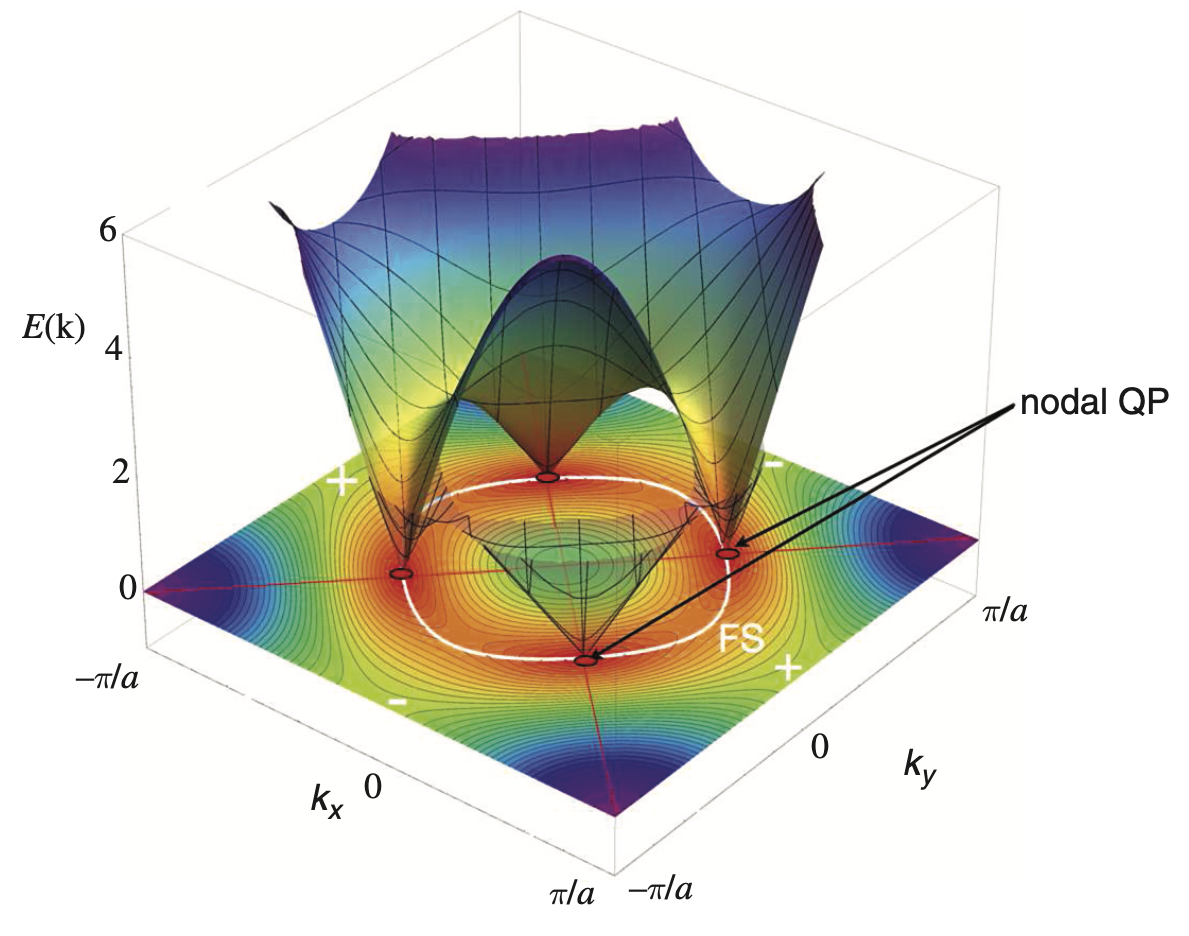
\includegraphics[width=0.6\textwidth]{notes/images/energy dispersion d-wave}
    \caption{}
    \label{fig:d-wave dispersion}
\end{figure}
\todo{What exactly is shown in the figure?}
It vanishes at intersections of nodes (where \(\Delta_{\vb{k}} = 0\)) and the Fermi surface (where \(\epsilon_{\vb{k}} = 0\)).
At these points the dispersion can be linearized, they form Dirac cones of excitations with a relativistic dispersion \todo{What is the exact dispersion?}.
We can approximately solve the gap equation and get
\begin{equation}
    \Delta_D (c_y - c_x) = \Delta_D (k_x^2 - k_y^2) = \Delta_0 \cos{(2\theta)}
\end{equation}
The dependence \(\Delta \propto \cos{(2\theta)}\) is typical for an \(l=2\) Cooper pair. \todo{How exactly typical? \(l=2\)?}\todo{Visualise that somehow?}
The quasiparticle energy is then
\begin{equation}
    E_{\vb{k}} = \sqrt{\epsilon_{\vb{k}}^2 + (\Delta_0 \cos{(2\theta)})^2}
\end{equation}
The d-wave density of states does not have a clear gap, but instead a V-shaped structure.
This linear DOS across the gap is due to the Dirac cones.
\begin{figure}[ht]
    \centering
    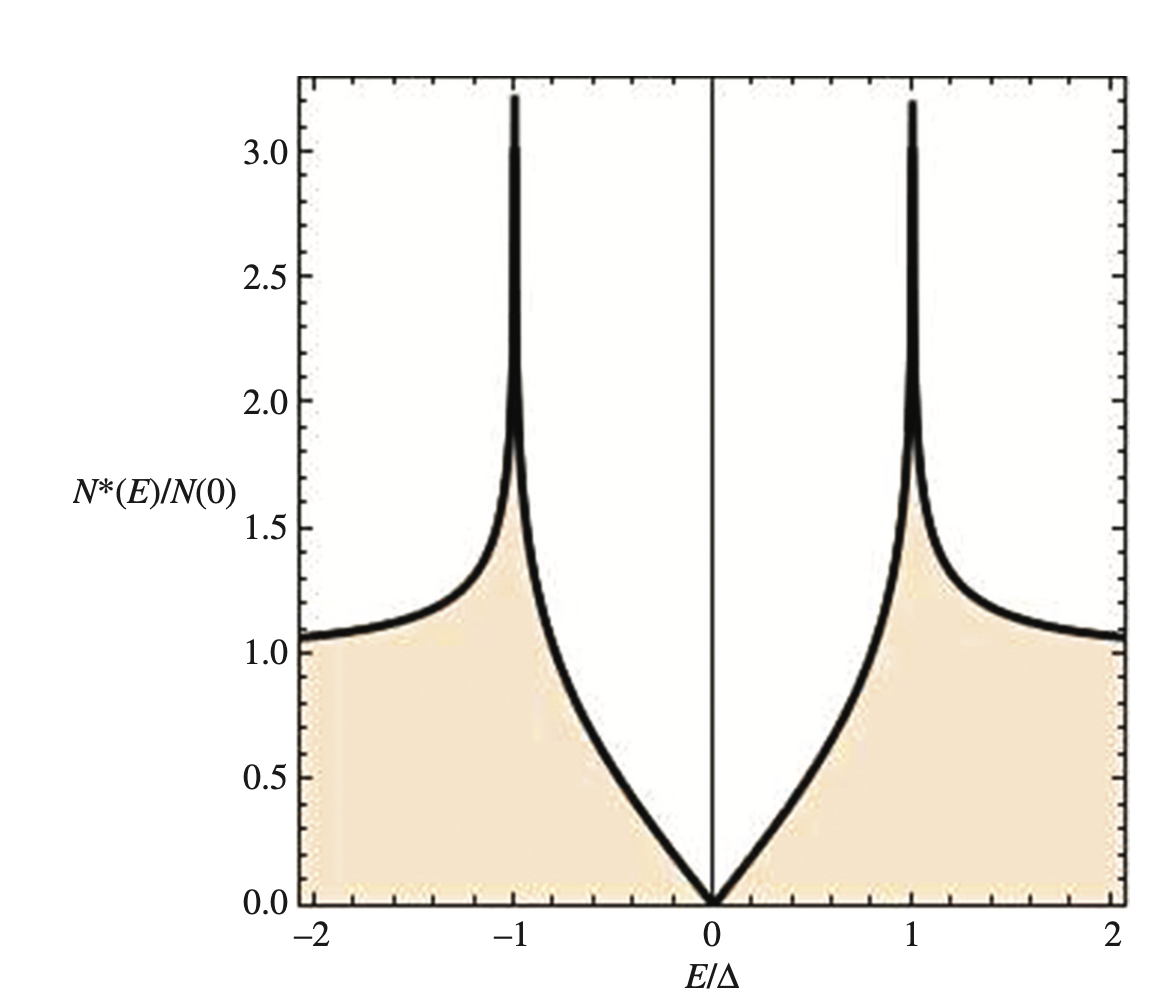
\includegraphics[width=0.6\textwidth]{notes/images/density of states d-wave}
    \caption{}
    \label{fig:d-wave density of states}
\end{figure}
\todo{How does the DOS compare with real materials? Do we have the V-shaped structure?}
